
\section{はじめに}
% \red{グラフ上の警邏問題を考えるにあたって,既存の結果との関連など}

1人または複数の巡査が所与の領域を動き回り,その領域内のあらゆる場所を十分な頻度で訪問することで,
これを守備,監督することを警邏(patrolling)という~\cite{czyzowicz2011boundary}.

警邏に関する研究には様々な問題設定があり,
例えば線分や閉路のような交わりの無い1次元的な領域のすべての点を警邏する
塀の警邏(Fence Patrolling)問題~\cite{czyzowicz2011boundary, chen2013fence}や,
より一般的なグラフで辺全体ではなく頂点を警備する警邏問題を考えることもできる~\cite{coene2011charlemagne}.
グラフと巡査が与えられて警邏可能かを判定する問題だけでなく,
全体を警邏可能な最小の巡査数を求める問題,
塀の警邏問題においてはなるべく長い塀を警邏する問題~\cite{czyzowicz2011boundary}や
全体の訪問の待ち時間の最大値を最小化する問題~\cite{chen2013fence},
頂点の警邏問題においては警備できる頂点数を最大化したり,さらに頂点に利得を設定しそれを最大化する問題,
{\timelimit}が頂点ごとに異なる場合~\cite{coene2011charlemagne}
も考えられている.

Coeneら~\cite{coene2011charlemagne}は,
辺の長さの与えられた無向グラフと
各頂点の持つ利得・放置可能時間,巡査の人数が与えられたとき,
グラフ上を最高速度が1である1人または複数の巡査が動きながら,
各頂点を訪問する間隔を
その点の{\timelimit}以内にしなければならない制約を満たしながら訪問し続けられる
頂点から得られる利得の合計を最大化するような点部分集合を求める警邏問題を考えた.
本稿ではこの問題を取り上げ,
多項式時間で解けるか否か未解決であった形状について調べる.
そのままの問題設定では解決できなかった部分については,
{\timelimit}の代わりに{\period}が与えられたときに,
最初の訪問時刻からその{\period}ごとの時刻は必ず訪問しなければならないという問題,
さらに最初の訪問時刻も指定される問題も考える.
与えられた入力に対して単に全点を警邏できるかを判定する問題 \decisionpp (Point Patrolling) と,
利得の合計を最大化する問題 \optpp を考える.
\decisionpp は \optpp により解けるので \optpp は \decisionpp 以上に難しいといえる.

他に,全点を警備できる最小の巡査数を求める問題も考えられるが,
頂点が $n$ 点のとき,巡査が $n$ 人いれば各頂点に1人ずつ停止させることで全点を警備できることから,
巡査数 $m = 1, \ldots, n$ について \decisionpp を解き
全点を警備できた最初の $m$ によって最小巡査数を求めることができ,
逆に巡査数最小化を解きその巡査数と \decisionpp の入力の巡査数の大小を比較することで
\decisionpp を判定できるので,
巡査数最小化は多項式時間帰着の関係において \decisionpp と同等である.




\subsection{問題設定の詳細}
頂点集合を $V = \set{ v_1, \ldots, v_n }$,
辺を $E \subseteq V \times V$, 
辺の長さを $d : E \to \N$ とする無向グラフ $G = (V,E,d)$ の上を
1人または複数人の点で表される巡査が速さ1以下で動きながら各頂点を訪問する.
各頂点 $v_i$ には利得 $p_i$ と{\timelimit} $q_i$ が与えられている.
ある頂点を警備できているとは,どの連続した2回の訪問も間隔がその点の{\timelimit}以内となるように
訪問し続けられることと定義する.
グラフ $G$ と利得 $p_1, \ldots, p_n$, {\timelimit} $q_1, \ldots, q_n$ と
巡査の人数 $m$ が与えられたときに,
警備される点から得られる利得の合計を最大化する問題を
\optpp と呼び,
グラフ $G$ と{\timelimit} $q_1, \ldots, q_n$ と巡査の人数 $m$ が与えられたときに,
$G$ の全点を警備できるかを判定する問題を \decisionpp と呼ぶことにする.
\decisionpp は全点を警邏する問題なので利得は無関係になっている.
巡査は2人以上同時に1つの点に存在してもよいし,
1つの点は複数人の巡査により交代で訪問して警備してもよいとする.
利得が0以下のものは警備する必要がないので最初に除外して利得はすべて正の整数であるとする.
{\timelimit}は非負整数とする.





\section{結果}


\subsection{既存の結果との関連と本稿の構成}
本稿ではCoeneらと同じ問題設定~\cite{coene2011charlemagne}を考える.
Coeneらは,
グラフの形状としてLine(線分),Circle(閉路),Star(星),Tree(木),一般のグラフを扱っていた.
Line は全ての頂点がある1つの線分上に存在するグラフ,
Circle は Line の両端がつなぐ辺を足したグラフのことである.
一般のグラフの場合,巡査が1人で利得・{\timelimit}がすべて等しいという最も簡単な場合でもNP困難であることが示されており,
Star, Tree については,巡査が1人で利得・{\timelimit}がすべて等しい場合のみには多項式時間アルゴリズムが存在するが,
それ以外の巡査が複数である場合や利得・{\timelimit}のいずれかが一般の場合はいずれもNP困難であることが示されている.
Line, Circle については巡査が1人の場合は多項式時間アルゴリズムが存在することが示されているが,
巡査が複数の場合に対する多項式時間アルゴリズムは間違っていた.
また,枝の長さがすべて等しい Star (本稿では UStar と呼ぶ) についても
Coeneら~\cite{coene2011charlemagne}が巡査1人で利得がすべて等しい場合にのみ触れており,
この場合は多項式時間アルゴリズムが存在すると述べているがこれも誤りであり,
さらに巡査が複数の場合などについても扱っていなかった.
以上のように,Coeneらの論文~\cite{coene2011charlemagne}で
既に Star のような単純な図形でもほとんどの場合でNP困難となっている一方,
Line で巡査が複数の場合や UStar のような単純な図形については
未解決の場合があるので本稿で調べることにした.

Coeneら~\cite{coene2011charlemagne}は,
Line で巡査が複数の場合,すべての巡査はある区間を往復運動しており,
そのうち任意の2つの区間は,互いに交わりの無い区間であるか,一方の区間がもう一方の区間に含まれるか
のいずれかであるというような最適解が存在すると述べているが,これは誤りであり
反例を\ref{subsec:Line_different_timelimit}章で述べる.
本稿ではLine については巡査が複数の場合について調べ,
まず,{\timelimit}がすべて等しいならば
多項式時間アルゴリズムが存在することを示した(定理\ref{theo:1_Line_multiple_Q_polytime}).
{\timelimit}が一般の場合については多項式時間アルゴリズムもNP困難性も示せなかったので,
{\timelimit}ではなく{\period}と最初の訪問時刻が与えられ,
最初の訪問時刻からその{\period}ごとの時刻は必ず訪問しなければならないという問題を考え,
アルゴリズムを示した(定理\ref{theo:2_Line_exact_finite}).

Star については上述のように多くの場合についてNP困難性が既に示されているが,
辺の長さが異なることが証明においても重要な役割を果たしており問題の難しさの一つの要因であると考えられ,
実際 UStar の場合は,{\timelimit}がすべて等しい場合については
巡査が複数でも多項式時間アルゴリズムを示すことができた(定理\ref{theo:3_UStar_multiple_Q_polytime}).

% しかしこちらも{\timelimit}が異なる場合については多項式時間アルゴリズムもNP困難性も示せなかったため,
% 先ほどと同様{\timelimit}ではなく{\period}と最初の訪問時刻が与えられる問題や
% 最初の訪問時刻は指定されず{\period}のみ与えられる問題を考え,
% 前者は \decisionpp には多項式時間アルゴリズム(定理\ref{theo:4_UStar_single_exact_starttime}),
% \optpp にはNP困難性の証明(定理\ref{theo:5_UStar_exact_starttime_NPhard})を与え,
% 後者は \decisionpp でもNP困難であることを示した(定理\ref{theo:6_UStar_exact_NPhard}).


% \subsection{形状}
% 本稿では Line, UStar という形状について考察する.
% Line は $E = \setmid{ (v_i, v_{i + 1}) }{ 1 \leq i \leq n - 1 }$ 
% で表される一直線上に点が並んだグラフであり,
% UStar は $E = \setmid{ (v_i, v_0) }{ 1 \leq i \leq n }$ 
% で表される星(すべての枝の端点の一方が根 $v_0$ であるような木,Star と呼ぶことにする)であって
% 辺の長さがすべて等しいグラフとする.
% Line, UStar も Coeneら~\cite{coene2011charlemagne} が扱っていた形状の一部であるが,
% 証明の誤りやまだ調べられていない状況が含まれるので,本稿で詳しく調べる.

以上をまとめた現在分かっている計算量を以下の表に示す.
% 巡査数の列の $1$ と $\geq 1$ はそれぞれ巡査が1人の場合と複数の場合を表す.
% {\timelimit}の列の $Q$ は,すべての点の周期が等しい $q_i = Q$ である場合,$\geq 0$ はそうでない場合を表す.
% 目的の列の $1$ は,すべての点の利得が等しい場合,$> 0$ はそうでない場合,
% Dは \decisionpp の場合を表す.
% 利得がすべて等しいならば単に点の数を最大化する問題に相当し $p_i = 1$ としてよい.
% Pは多項式時間アルゴリズムが存在すること,
?の部分は未解決であることを表しており,括弧内は対応する定理番号を表す.
太字が今回示した部分である.


\begin{table}[h]
	\centering
	\caption{\optpp の計算量一覧\label{tab:Patrol}}
	\begin{tabular}{|c|c||c|c|c|}
		\hline {\timelimit}  & 巡査数  & Line  & UStar  & Star \\
		\hline すべて等しい & $1$        & P             & {\bf P}        & NP困難($\star 1$)  \\
		\hline すべて等しい & 複数 
			& {\bf P} (\ref{theo:1_Line_multiple_Q_polytime})
			& {\bf P} (\ref{theo:3_UStar_multiple_Q_polytime})
			& NP困難 \\
		\hline 一般の場合 & $1$  & P             & ? ($\star 3$)  & NP困難  \\
		\hline 一般の場合 & 複数 & ? ($\star 2$) & ? ($\star 4$)  & NP困難  \\
		\hline
	\end{tabular}
\end{table}

$\star 1$ は利得がすべて等しいならば辺の短いものから
移動時間の合計が $Q$ を超えない範囲で選べばよいのでPとなる~\cite{coene2011charlemagne}.

?のうち
Line の $\star 2$ の部分は{\timelimit}ではなく{\period}として最初の訪問時刻も指定される問題ならば
定理\ref{theo:2_Line_exact_finite}の特殊な場合となり,
この定理で述べるアルゴリズムにより解ける.
UStar で
{\timelimit}ではなく{\period}として最初の訪問時刻も指定される問題ならば
$\star 3$ の部分に対応する巡査が1人の場合は \decisionpp ならば
定理\ref{theo:4_UStar_single_exact_starttime}のようにPとなり,
一方 \optpp は巡査が1人でも定理\ref{theo:5_UStar_exact_starttime_NPhard}のようにNP困難となる($\star 3,4$ の部分に対応).
また,同じ設定で最初の訪問時刻は指定されない場合だと
\decisionpp でも定理\ref{theo:6_UStar_exact_NPhard}のようにNP困難となる($\star 3,4$ の部分に対応).

% 巡査は点を訪問するときに一定時間 $w$ ほどその点に留まる必要があるという問題も考えられるが,
% 元のグラフの点の位置から長さ $w/2$ の枝を生やしてその末端に点を配置すれば,
% その点の訪問のためにかかる時間を $w$ 増やすことができるので,滞在時間の無い問題に帰着できる.


% \begin{theo}
% 	\label{theo:1_Line_multiple_Q_polytime}
% 	$G$ が Line で{\timelimit}がすべて等しい場合,
% 	巡査が複数で利得が異なっていて \optpp でも
% 	多項式時間アルゴリズムが存在する.
% \end{theo}


% \begin{theo}
% 	\label{theo:2_Line_exact_finite}
% 	$G$ が Line で,
% 	各点 $x_i$ に対し訪問しなければならない時刻 $t_{i_1}, t_{i_2}, \ldots, t_{i_{N_i}}$ が有限個指定されているとき,
% 	巡査が複数でも,
% 	$X = \dbigcup_{i = 1}^n \dbigcup_k^{N_i} \set{(t_{i_k}, x_i)}$
% 	として $O( |X| \log |X| )$ で \decisionpp を解くことができる.
% \end{theo}


% \begin{theo}
% 	\label{theo:3_UStar_multiple_Q_polytime}
% 	$G$ が UStar で周期がすべて等しい場合,
% 	巡査が複数で利得が異なっていて \optpp でも
% 	多項式時間アルゴリズムが存在する.
% \end{theo}

% \begin{theo}
% 	\label{theo:4_UStar_single_exact_starttime}
% 	$G$ が UStar で巡査が1人,
% 	最初の訪問時刻と{\period}が与えられる場合,
% 	{\period}は異なっていても
% 	\decisionpp には多項式時間アルゴリズムが存在する.
% \end{theo}

% \begin{theo}
% 	\label{theo:5_UStar_exact_starttime_NPhard}
% 	$G$ が UStar で,
% 	最初の訪問時刻と{\period}が与えられる場合,
% 	巡査が1人で利得がすべて等しい場合でも,
% 	\optpp はNP困難である.
% \end{theo}

% \begin{theo}
% 	\label{theo:6_UStar_exact_NPhard}
% 	$G$ が UStar で,
% 	周期ちょうど毎の時刻に訪問しなければならないとき,
% 	巡査が1人で \decisionpp でもNP困難である.
% \end{theo}






% 表\ref{tab:Patrol}の?の部分について考察中に得られた結果として,
% 最初の訪問時刻指定されていて,かつ周期 $q_i$ ちょうど毎の時刻には訪問しなければならない
% (それ以外の時刻に訪問することは許す)という別種の問題設定を考えた場合,
% Line については定理\ref{theo:2_Line_exact_finite}のような貪欲アルゴリズムが存在し,
% UStarについては\decisionpp については定理\ref{theo:4_UStar_single_exact_starttime}のような多項式時間アルゴリズム,
% \optpp については定理\ref{theo:5_UStar_exact_starttime_NPhard}のようなNP困難性を示した.
% さらに,最初の訪問時刻は指定せずに周期のみちょうどにした問題では,
% UStar で周期が異なる場合は \decisionpp も \optpp もNP困難であることを示した(定理 \ref{theo:6_UStar_exact_NPhard}).
% 表 \ref{tab:Patrol2} の $r_i$ の列は最初の訪問時刻を与えるかどうかを表す.

% \begin{table}[h]
% 	\centering
% 	\caption{警邏問題の計算量一覧(周期ちょうどで訪問)\label{tab:Patrol2}}
% 	\begin{tabular}{|c|c|c||c|c|}
% 		\hline $r_i$     & $m$      &             & Line                             & UStar \\
% 		\hline given     & $1$      & \decisionpp & (\ref{theo:2_Line_exact_finite}) & P (\ref{theo:4_UStar_single_exact_starttime}) \\
% 		\hline given     & $1$      & \optpp      & ?                                & NP困難 (\ref{theo:5_UStar_exact_starttime_NPhard}) \\
% 		\hline given     & $\geq 1$ & \decisionpp & (\ref{theo:2_Line_exact_finite}) & ?     \\
% 		\hline given     & $\geq 1$ & \optpp      & ?                                & ?     \\
% 		\hline not given & $1$      & \decisionpp & ?                                & NP困難 (\ref{theo:6_UStar_exact_NPhard}) \\
% 		\hline not given & $1$      & \optpp      & ?                                & NP困難 (\ref{theo:6_UStar_exact_NPhard}) \\
% 		\hline not given & $\geq 1$ & \decisionpp & ?                                & NP困難 (\ref{theo:6_UStar_exact_NPhard}) \\
% 		\hline not given & $\geq 1$ & \optpp      & ?                                & NP困難 (\ref{theo:6_UStar_exact_NPhard}) \\
% 		\hline
% 	\end{tabular}
% \end{table}





\section{Line}

$G$ が Line の場合は実直線上にすべての点を置くことができるので,
それぞれの座標を $x_1, x_2, \ldots, x_n$ とする.
また,添え字は $x_1 \leq x_2 \leq \cdots \leq x_n$ としておく.

巡査が1人の場合についてはCoeneら~\cite{coene2013balancing}
により多項式時間アルゴリズムが示されているので,
巡査が複数の場合を考える.

巡査達の能力は皆同じなので,
巡査がすれ違うような動きはお互いの動きを交換し引き返すような動き方にすることができる.
これにより,巡査は初期配置の $x$ 軸上の順番を保って動くとしてよいことが言える.
ある実行可能解 $A$ についてこのような変換を行ったものを $A^*$ と表すことにする.



\subsection{{\timelimit}がすべて等しい場合}
まず{\timelimit}がすべて等しい場合を考える.
この場合,同じ位置に複数の点が存在するとき,そのどれか1つを警備できるならばすべて警備できるので,
それらの合計の利得をもつ新たな1つの点にまとめることができる.
よってここでは $x_1 < x_2 < \cdots < x_n$ となっているとして進める.

% 巡査が1人の場合については多項式時間アルゴリズムが既に示されているので,
% 巡査が複数の場合について次の定理を示す.

\begin{theo}
	\label{theo:1_Line_multiple_Q_polytime}
	$G$ が Line で{\timelimit}がすべて等しい場合,
	巡査が複数で \optpp でも
	多項式時間アルゴリズムが存在する.
\end{theo}


初めに次の補題を示す.

\begin{lemm}
	\label{lemm:MultiplePatrolOnLine_3}
	ある1人の巡査 $s$ のみにより警備されている点 $x_i$ が存在するとき,
	$s$ が動ける範囲は $\abs{ x - x_i } \leq q_i / 2$ となる.
\end{lemm}

\begin{proof}[証明]
	もし $s$ が $\abs{ x_{out} - x_i } > q_i /2$ であるような位置 $x_{out}$ に
	行くことがあるとすると,
	$s$ が最後に $x_i$ を出発してからの時間と,
	次に $x_i$ に戻るまでの時間を合わせた時間 $t$ は
	$t > 2 \abs{ x_{out} - x_i} > q_i$
	となり,
	$x_i$ は $s$ 以外の巡査により訪問されていないので
	$x_i$ を警備できていないことになり矛盾する.
\end{proof}



\begin{lemm}
	\label{lemm:MultiplePatrolOnLine_2}
	巡査が複数,$G$ が Line, $q_i = Q$ の警邏問題に対するある実行可能解 $A$ について,
	各巡査がそれぞれ独立で両端に点があるような区間を往復する実行可能解であって
	$A$ 以上の利得を得られるようなものが存在する.
\end{lemm}

\begin{proof}[証明]
	$A$ で警備する点の集合を
	$V_S = \set{ v_1', v_2', \ldots, v_k' }$ $( x_1' < x_2' < \cdots < x_k' )$
	とする.
	まず $A$ を巡査の初期順序を保つ動き $A^*$ に変換し,
	それらを $x$ 軸上の左側から $s_1, s_2, \ldots, s_m$ とする.
	さらに,$x < x_1'$ を動くものはその時間 $x_1'$ で待機するようにしても損をしないため
	($x_k' < x$ も同様),
	すべての巡査は区間 $[x_1', x_k']$ を動くように変換できる.

	まず $x_1'$ に注目する.
	いま,巡査順序を保つ $A^*$ に変換しており,
	巡査は $x_1'$ より左には進まないように変換しているので,
	$x_1'$ に $s_1$ 以外の巡査が訪れるときは必ず $s_1$ が $x_1'$ に存在することになる.
	よって,$s_1$ 以外の巡査は $x_1'$ を訪れずに $x_2' \leq x$ を動くようにしてよい.

	補題\ref{lemm:MultiplePatrolOnLine_3}により $s_1$ の可動範囲は
	$[x_1', x_1' + Q/2]$ となるが,
	$s_1$ はこの区間を往復することによりこの区間に存在するすべての点を警備できるので,
	この区間 $[x_1', x_1' + Q/2]$ に含まれる点を $s_1$ 以外の巡査が警備する必要はない.
	$V_S$ の点のうち
	$x$ より左にあり最も $x$ に近い点の位置を
	$l(x)$% := \dmax_{ \setmid{ v_i \in V_S }{ x_i \leq x } } x_i$, 
	$x$ より右にあり最も $x$ に近い点の位置を
	$r(x)$% := \dmin_{ \setmid{ v_i \in V_S }{ x \leq x_i } } x_i$, 
	と書くことにすると,
	$s_1$ は区間 $[x_1', l(x_1' + Q/2)]$ を往復すればよく,
	$s_2, \ldots, s_m$ のうち
	$[x_1', r(x_1' + Q/2))$ を動いていた巡査は
	$r(x_1' + Q/2)$ でその時間待機するようにしてよい.

	このような変換の後,
	$r(x_1' + Q/2)$ を警備している最も添え字の若い巡査を $s_j$ とすると,
	$s_j, s_{j + 1}, \ldots, s_m$ と区間 $[r(x_1' + Q/2), x_k']$
	に存在する点について,$s_1$ のときと同様の変換をさらに行うことができる.
	これを最後まで繰り返すと,
	すべての巡査がそれぞれ両端に点が存在するような
	独立な区間を往復(または1点で停止)するような動きに変換できる.
	この変換で $A$ で警備していた点はすべて警備できているので $A$ 以上の利得が得られている.
\end{proof}


以上により,各巡査の動きとしては
区間 $[x_i, l(x_i + Q/2)]$ を往復するもののみを考えれば良いため,
$n$ 個の区間 $[x_i, l(x_i + Q/2)] \quad (i = 1, 2, \ldots, n)$ から
得られる利得の大きい順に $m$ 個の重複のない区間を選ぶことで最適解が得られる.
$n$ 個の区間 $I_i := [x_i, l(x_i + Q/2)]$ について
その区間に含まれる点から得られる利得の合計 $P_i$ を求めておき,
重み付き区間の選択問題で選べる区間数が $m$ 個以下という制限付きの場合を解けばよい.

まず $x_1, \ldots, x_n$ はソートしておく.
前半の $P_i$ の求め方だが,
$x_1, \ldots, x_n$ を $x$ 軸上に並べ,
幅 $Q/2$ の区間を左から動かしていきながら
点 $x_i$ がその区間を出入りするごとにこの区間に含まれる点の利得の合計を更新していくことで計算できる.
これは,
$x_1, \ldots, x_n$ と $(x_1 + Q/2), \ldots, (x_n + Q/2)$ を
先頭から見て小さい方から1つずつ取り出していき,
$x_i$ なら $p \gets p + p_i$, 
$x_i + Q/2$ なら $P_i \gets p$; $p \gets p - p_i$
という操作をしていくことで計算できる.
$p$ は今見ている幅 $Q/2$ の区間に含まれる点の利得の合計を表す一時変数で,最初に0で初期化する.


後半の,重複のない $m$ 個の区間を選び重みの和を最大化する問題は,
以下の漸化式\ref{eq:MultiplePatrolOnLine_DP}に従う動的計画法で
$m \times n$ の表を左上から計算することにより $O(mn)$ で
最適な区間を選択できる.
$h(j)$ は,区間 $I_j$ より左にある交わらない区間のうち最も右にあるものの添え字を返すもので,
$1 \leq j \leq n$ について $O(n)$ の前計算で得られる.
$OPT(i,j)$ は,区間 $I_1, \ldots, I_j$ から 最大 $i$ 個の区間を選ぶときの
重みの合計の最大値を表す.
$OPT(m,n)$ が求めたい利得の最大値となる.
選ばれた区間も表をトレースバックすることにより再計算でき,
巡査は互いに独立にそれらの区間を往復すればよい.

\begin{equation}
	\label{eq:MultiplePatrolOnLine_DP}
	OPT(i, j) = 
	\begin{cases}
		0 & \IF i = 0 \\
		\max
		\begin{cases}
			OPT(i, j - 1) \\
			P_j + OPT(i - 1, h(j))
		\end{cases}
		 & \IF i \neq 0 \\
	\end{cases}
\end{equation}

この算法の計算量は最初のソートも含めて全体で $O(n \log n + nm)$ である.
これで定理 \ref{theo:1_Line_multiple_Q_polytime} が示された.




\subsection{{\timelimit}が一般の場合}
\label{subsec:Line_different_timelimit}

次に,{\timelimit}が一般の場合を考える.
こちらは計算量を決定できなかったが,
この場合の難しさを示唆するいくつかの例を示す.

点の{\timelimit}がすべて $Q$ であるときは,巡査は各々の区間を独立に往復すればよかったが,{\timelimit}が任意の場合,
動く範囲に交わりがあり往復でもない動きが最適となる次のような例が存在する.
図\ref{tikz:multiserver_example}は
巡査の軌跡(各時刻 $t$ における巡査の位置 $x$ を表す関数 $f : t \mapsto x$ を $t$-$x$ 平面に描いたときのグラフ)
を横軸を点の位置 $x$, 縦軸を時刻として $t$-$x$ 平面に書いたものであるが,
この例では,左から $q_1 = 10$, $q_2 = 2$, $q_3 = 2$, $q_4 = 10$ である4つの点
が存在するとき,図のような動き方をしなければ全点を警邏するのに $3$ 人目の巡査が必要になる.

\begin{figure}[h]
	\centering
	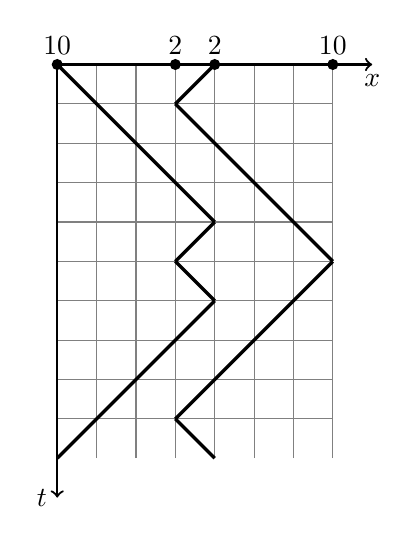
\begin{tikzpicture}
		\draw [help lines,thin,step=5mm] (0,5) grid (3.5,10);
		\draw[thick, ->] (0,10) -- (4,10) node [below] {$x$};
		\draw[thick, ->] (0,10) -- (0,4.5) node [left] {$t$};

		\fill ( 0  , 10) coordinate (c1) circle (2pt) node [above] {10};
		\fill ( 1.5, 10) coordinate (c2) circle (2pt) node [above] { 2};
		\fill ( 2  , 10) coordinate (c3) circle (2pt) node [above] { 2};
		\fill ( 3.5, 10) coordinate (c4) circle (2pt) node [above] {10};

		\draw[very thick,-] ( 0  ,10  )--( 2  , 8  );
		\draw[very thick,-] ( 2  , 8  )--( 1.5, 7.5);
		\draw[very thick,-] ( 1.5, 7.5)--( 2  , 7  );
		\draw[very thick,-] ( 2  , 7  )--( 0  , 5  );

		\draw[very thick,-] ( 2  ,10  )--( 1.5, 9.5);
		\draw[very thick,-] ( 1.5, 9.5)--( 3.5, 7.5);
		\draw[very thick,-] ( 3.5, 7.5)--( 1.5, 5.5);
		\draw[very thick,-] ( 1.5, 5.5)--( 2  , 5  );
	\end{tikzpicture}
	\caption{複数人の巡査が複雑に動く例 \label{tikz:multiserver_example}}
\end{figure}


この例で最も左を動く $s_1$ は「可能な限り右に手伝いに行く」動き方(後で数学的に定義する)をしているので,
各巡査の動きは最も左を動く $s_1$ から順に
「可能な限り右に手伝いに行く」動き方により貪欲決定してよいのではないかという予想を立てたが,
これも成り立たない次のような例が存在する.
図\ref{tikz:multiserver_example2}のように,
左から $q_1 = 8$, $q_2 = 2$, $q_3 = 2$, $q_4 = 3$, $q_5 = 6$ である $5$ つの点
が存在するとき,
左図のように $s_1$ が可能な限り右に行くような動きをしてしまうと
$v_2,v_3,v_5$ の{\timelimit}を満たす動きが左図のようなものになり
($s_1$ の動きを図のように決めると $v_2$ と $v_5$ の訪問のために $s_2$ の動きも図のように決まってしまう),
$v_4$ が{\timelimit} $3$ 以内に訪問されなくなってしまうので $3$ 人目の巡査が必要になるが,
右図のようにあえて{\timelimit} $6$ で $v_1$ に戻るような動き方をすれば $2$ 人の巡査で5つの点を警備できる.


\begin{figure}[h]
	\centering
	\begin{tabular}{cc}
	
	\begin{minipage}{0.5\hsize}
		\centering
		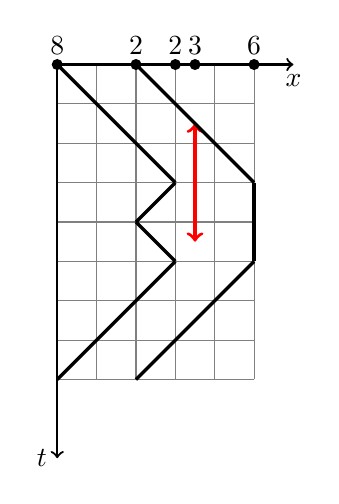
\begin{tikzpicture}
			\draw [help lines,thin,step=5mm] (0,-4) grid (2.5,0);
			\draw[thick, ->] (0,0) -- (3,0) node [below] {$x$};
			\draw[thick, ->] (0,0) -- (0,-5) node [left] {$t$};

			\fill ( 0   , 0) coordinate (c1) circle (2pt) node [above] {8};
			\fill ( 1   , 0) coordinate (c2) circle (2pt) node [above] {2};
			\fill ( 1.5 , 0) coordinate (c3) circle (2pt) node [above] {2};
			\fill ( 1.75, 0) coordinate (c4) circle (2pt) node [above] {3};
			\fill ( 2.5 , 0) coordinate (c5) circle (2pt) node [above] {6};

			\draw[very thick,red,<->] (1.75,-0.75)--(1.75,-2.25);

			\draw[very thick,-] ( 0  , 0  )--( 1.5,-1.5);
			\draw[very thick,-] ( 1.5,-1.5)--( 1  ,-2  );
			\draw[very thick,-] ( 1  ,-2  )--( 1.5,-2.5);
			\draw[very thick,-] ( 1.5,-2.5)--( 0  ,-4  );

			\draw[very thick,-] ( 1  , 0  )--( 2.5,-1.5);
			\draw[very thick,-] ( 2.5,-1.5)--( 2.5,-2.5);
			\draw[very thick,-] ( 2.5,-2.5)--( 1  ,-4  );
		\end{tikzpicture}
	\end{minipage}
	
	\begin{minipage}{0.5\hsize}
		\centering
		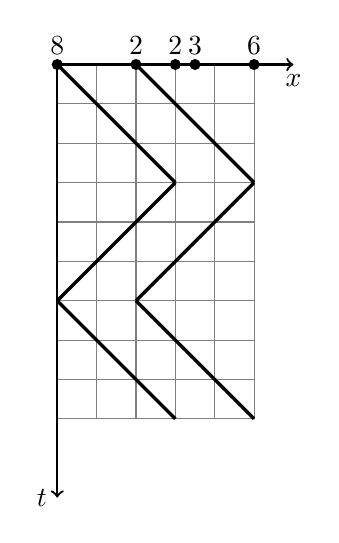
\begin{tikzpicture}
			\draw [help lines,thin,step=5mm] (0,-4.5) grid (2.5,0);
			\draw[thick, ->] (0,0) -- (3,0) node [below] {$x$};
			\draw[thick, ->] (0,0) -- (0,-5.5) node [left] {$t$};

			\fill ( 0   , 0) coordinate (c1) circle (2pt) node [above] {8};
			\fill ( 1   , 0) coordinate (c2) circle (2pt) node [above] {2};
			\fill ( 1.5 , 0) coordinate (c3) circle (2pt) node [above] {2};
			\fill ( 1.75, 0) coordinate (c4) circle (2pt) node [above] {3};
			\fill ( 2.5 , 0) coordinate (c5) circle (2pt) node [above] {6};

			\draw[very thick,-] ( 0  , 0  )--( 1.5,-1.5);
			\draw[very thick,-] ( 1.5,-1.5)--( 0  ,-3  );
			\draw[very thick,-] ( 0  ,-3  )--( 1.5,-4.5);
			\draw[very thick,-] ( 1  , 0  )--( 2.5,-1.5);
			\draw[very thick,-] ( 2.5,-1.5)--( 1  ,-3  );
			\draw[very thick,-] ( 1  ,-3  )--( 2.5,-4.5);
		\end{tikzpicture}
	\end{minipage}
	
	\end{tabular}
	\caption{「可能な限り右に手伝いに行く」戦略が失敗する例 \label{tikz:multiserver_example2}}
\end{figure}




\subsubsection{最初の訪問時刻指定,周期ちょうど毎に訪問}

各頂点の{\timelimit}とは,連続する2回の訪問の間隔の上限であったが,
それにより,図\ref{tikz:multiserver_example2}の例のようにあえて{\timelimit}8の点を時間6毎に訪問
する方が良いという,左端から巡査の動きを貪欲に決定できないという難しさが生じてしまった.
{\timelimit}の代わりに{\period}と最初の訪問時刻が与えられたときに,
その最初の訪問時刻からその{\period}ごとの時刻は必ず訪問しなければならないという問題を考えてみる.
すると,この設定では,左側から巡査を割り当て,「可能な限り右に行く」動き方をさせることにより
全点の警備を考える \decisionpp では最適解が得られることを以下のように示すことができる.
実際にはより一般的に,時刻 $t$ と位置 $x$ について
$t$-$x$ 平面に訪問しなければならない位置と時刻を表す点がすべて与えられている問題についての
次の定理により示される.


\begin{theo}
	\label{theo:2_Line_exact_finite}
	$G$ が Line で,
	各頂点 $x_i$ に対し訪問しなければならない時刻 $t_{i_1}, t_{i_2}, \ldots, t_{i_{N_i}}$ が有限個指定されているとき,
	巡査が複数でも,
	$X = \dbigcup_{i = 1}^n \dbigcup_k^{N_i} \set{(t_{i_k}, x_i)}$
	として $O( |X| \log |X| )$ で \decisionpp を解くことができる.
\end{theo}

まず次の補題を示す.

\begin{lemm}
	\label{lemm:xt_decided_1}
	各頂点 $x_i$ について,訪問すべき時刻の列
	が指定されているとき,
	$s_1, s_2, \ldots$ を順に「可能な限り右に行く動き方」により動きを決定することで
	\decisionpp の最適解を得られる.
\end{lemm}



\begin{defi}
	$t$-$x$ 平面において,点 $a = (t_a,x_a)$ に対して
	\begin{alignat*}{3}
	R(a)
	&:= \setmid{(t,x)}{ -x + x_a + t_a < t < x - x_a + t_a } \\
	L(a)
	&:= \setmid{(t,x)}{ (t,x) \not\in R(a) }
	\end{alignat*}
	と定義する.
	$R(a)$ を $R(t_a,x_a)$ のようにも書くことにする.
	\begin{figure}[h]
		\centering
		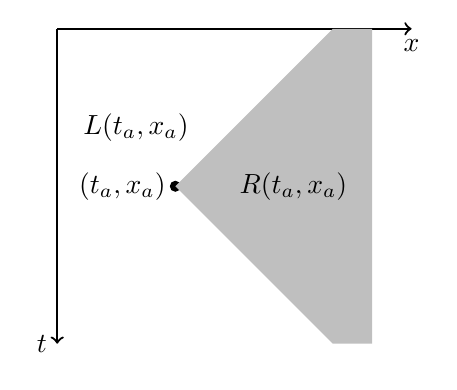
\begin{tikzpicture}
			% \draw [help lines, thin,step=10mm] (0,-5.5) grid (5.5,0);
			\draw[thick, ->] (0,0) -- (4.5, 0) node [below] {$x$};
			\draw[thick, ->] (0,0) -- (0,-4) node [left] {$t$};

			\fill ( 1.5,-2) coordinate (a) circle (2pt) node [left] {$(t_a,x_a)$};

			\fill [fill=lightgray]
				(a)--(3.5,0)--(4,0)--(4,-4)--(3.5,-4)--(a);

			\node (L) at (1,-1.25) {$L(t_a,x_a)$};
			\node (R) at (3,-2) {$R(t_a,x_a)$};
		\end{tikzpicture}
		\caption{$L(t_a,x_a)$ と $R(t_a,x_a)$ の定義 \label{tikz:defLR}}
	\end{figure}
\end{defi}


\begin{lemm}
	\label{lemm:xt_decided_2}
	巡査 $s$ の軌跡が $t$-$x$ 平面上のある点 $(t_a,x_a)$ を通るとき,
	$s$ の軌跡は $L(t_a,x_a)$ に含まれる ($R(t_a,x_a)$ を通らない).
\end{lemm}

\begin{proof}[証明]
	$s$ の軌跡が $(t_a,x_a)$ と $(t_b,x_b) \in R(t_a,x_a)$ を通るとする.
	$(t_b, x_b) \in R$ より
	\begin{equation}
		\label{eq:lemm:xt_decided_2}
		-x_b + x_a + t_a < t_b < x_b - x_a + t_a
	\end{equation}
	が成り立つ.
	$t_b = t_a$ のときは,式\ref{eq:lemm:xt_decided_2}から $x_b > x_a$ となり,
	$s$ が同時に異なる2点に存在することはできないので矛盾.
	$t_b < t_a$ のとき,巡査の速さが1以下であることから,
	$s$ が $x = x_b$ から $x = x_a$ に移動するのには少なくとも
	$\abs{x_b - x_a} = x_b - x_a$ 時間かかるので,
	時刻 $t_b$ 以降で $x_a$ に最初に到達する時刻 $t_a$ は
	$t_a \geq t_b + x_b - x_a$ を満たすが,
	これは 式\ref{eq:lemm:xt_decided_2}に矛盾する.
	$t_b > t_a$ のときも同様.
	% \begin{enumerate}[(i)]
	% 	\item $t_b = t_a$ のときは,式\ref{eq:lemm:xt_decided_2}から $x_b > x_a$ となり,
	% 	$s$ が同時に異なる2点に存在することはできないので矛盾.
	% 	\item $t_b < t_a$ のとき,巡査の速さが1以下であることから,
	% 	$s$ が $x = x_b$ から $x = x_a$ に移動するのには少なくとも
	% 	$\abs{x_b - x_a} = x_b - x_a$ 時間かかるので,
	% 	時刻 $t_b$ 以降で $x_a$ に最初に到達する時刻 $t_a$ は
	% 	$t_a \geq t_b + x_b - x_a$ を満たすが,
	% 	これは 式\ref{eq:lemm:xt_decided_2}に矛盾する.
	% 	\item $t_b > t_a$ のときも(ii)と同様.
	% \end{enumerate}

	よって,$s$ は $R(t_a,x_a)$ の点を通ることはできないので,
	$s$ の軌跡は $L(t_a,x_a)$ に含まれる.
\end{proof}


$t$-$x$ 平面上の点の集合 $X'$ が与えられ,
何人かの巡査により $X'$ の点すべてを通る必要があるとする.
$X' \neq \emptyset$ ならば,
巡査 $s_1$ を1人用意し,$X'$ を担当する巡査の中で最も左を動くものとする.
このとき,次の補題が成り立つ.


\begin{lemm}
	\label{lemm:xt_decided_2_3}
	$s_1$ の軌跡は $\dbigcap_{a \in X'} L(a)$ に含まれる.
\end{lemm}


\begin{proof}[証明]
	もし $s_1$ の軌跡が $\dbigcup_{a \in X'} R(a)$ の点 $b = (t_b,x_b)$ を通るとすると,
	ある $a = (t_a,x_a) \in X'$ が存在して $b \in R(a)$ であるが,
	このとき補題\ref{lemm:xt_decided_2}によると
	$s_1$ の軌跡は $a$ を通ることができない.
	すると,この $a$ を通る巡査 $s_2$ が新たに必要になるが,
	時刻 $t_a$ において $s_1$ は $x \geq x_b - \abs{t_b - t_a}$ の領域に存在するため,
	$t_b < t_a$ ならば,
	式\ref{eq:lemm:xt_decided_2}から
	$x \geq x_b - \abs{t_b - t_a} = x_b + t_b - t_a > x_a$,
	$t_b = t_a$ ならば,
	式\ref{eq:lemm:xt_decided_2}から
	$x \geq x_b > x_a$,
	$t_b > t_a$ ならば,
	式\ref{eq:lemm:xt_decided_2}から
	$x \geq x_b - \abs{t_b - t_a} = x_b - t_b + t_a > x_a$,
	% \begin{itemize}
	% 	\item $t_b < t_a$ ならば,
	% 	式\ref{eq:lemm:xt_decided_2}から
	% 	$x \geq x_b - \abs{t_b - t_a} = x_b + t_b - t_a > x_a$.
	% 	\item $t_b = t_a$ ならば,
	% 	式\ref{eq:lemm:xt_decided_2}から
	% 	$x \geq x_b > x_a$.
	% 	\item $t_b > t_a$ ならば,
	% 	式\ref{eq:lemm:xt_decided_2}から
	% 	$x \geq x_b - \abs{t_b - t_a} = x_b - t_b + t_a > x_a$.
	% \end{itemize}
	より,時刻 $t_b$ において $s_2$ は $s_1$ より左に存在することになる.
	これは $s_1$ を最も左側にある巡査にしたことに矛盾する.
	よって,最も左側の巡査 $s_1$ の軌跡は
	$\dbigcup_{a \in X'} R(a)$ の点を含まないので,
	$\dbigcap_{a \in X'} L(a)$ に含まれることが言える.
\end{proof}



\begin{lemm}
	\label{lemm:xt_decided_3}
	$t$-$x$ 平面上の点の集合 $X'$ に対し,
	$\dbigcap_{a \in X'} L(a)$ の(右の)境界線上にある点の集合を
	\[
		B(X')
		:= \setmid{ b \in X'}{ b \in \bigcap_{a \in X'} L(a) }
		= X' \cap \bigcap_{a \in X'}L(a)
	\]
	と表す.
	$X'$ を訪問する巡査のうち最も左にあるものを $s_1$ とすると,
	$s_1$ はその軌跡が $\dbigcap_{a \in X'} L(a)$ の(右側の)境界と一致する動きが最適であり,
	これにより $B(X')$ の点全体を担当することができる(これを「可能な限り右に行く動き」と定義する).
\end{lemm}


\begin{proof}[証明]
	補題\ref{lemm:xt_decided_2}より,$s_1$ の軌跡は
	$\dbigcap_{a \in X'} L(a)$ に含まれるので,
	$s_1$ が通ることができる点全体は
	$B(X')$ の点の部分集合となる.
	逆に,$s_1$ は $B(X')$ の点すべてを通ることができる.
	なぜならば,$\dbigcap_{a \in X'} L(a)$ の境界線は常に
	傾きが $\pm 1$ であるため,$B(X')$ の点のうち時刻の最も早い点から
	出発して境界線上を動くことにより
	$B(X')$ の点すべてを通ることができるためである.

	また,$B(X')$ の点をすべて通る動き方は最適である.
	なぜならば,$B(X')$ のうち通らない点がある場合,それらの点の集合を $X''$ と置くと,
	$X' \setminus B(X') \subseteq X' \cup X'' \cup (X' \setminus B(X'))$ より
	$X'' \cup (X' \setminus B(X'))$ の点すべてを通る巡査達の動きにより
	$X' \setminus B(X')$ 全体を通ることができるので,
	$B(X')$ をすべて $s_1$ が通ることで損をしないからである.
\end{proof}


以上より,定理\ref{lemm:xt_decided_1}に戻ると,
\[
X_i := 
\begin{cases}
	X & i = 1 \\
	X_{i - 1} \setminus B(X_{i - 1}) & i \geq 2
\end{cases}
\]
として,
$X_i$ が空集合になるまで $i = 1$ から順に $B(X_i)$ を巡査 $s_i$ が担当するようにすれば,
最適解が得られる.
これで定理 \ref{lemm:xt_decided_1} が示された.

この定理により得られた結果は
この問題設定に対しては巡査を左から可能な限り右に行く動き方で割り当てていけば良いということを
数学的に示したものであるが,
$X$ が無限集合のときは有限の手続きにより $X$ 全体を通る巡査数を求めることができるとは限らない.
$X$ が時刻方向に周期的になっている場合などのように
有限集合で考えてよい場合は $N := |X|$ 以下の手順により $O(N \log N)$ で
$t$-$x$ 平面上の巡査達の軌跡を描くことができる.

まず,$X$ の各頂点の元の $t$-$x$ 座標系での表示を
$45^\circ$ 反時計回りに回転した $u$-$y$ 座標系での表示に変換する.
% すなわち,各点 $(t_i, x_i)$ を以下のように $(u_i, y_i)$ に変換する.
% \begin{align*}
% 	\begin{pmatrix}
% 		u_i \\ y_i
% 	\end{pmatrix}
% 	&=
% 	\begin{pmatrix}
% 		\cos(-45^\circ) & - \sin(-45^\circ) \\
% 		\sin(-45^\circ) &   \cos(-45^\circ)
% 	\end{pmatrix}
% 	\begin{pmatrix}
% 		t_i \\ x_i
% 	\end{pmatrix} \\
% 	&=
% 	\frc{\sqrt{2}}
% 	\begin{pmatrix}
% 		1  & 1 \\
% 		-1 & 1
% 	\end{pmatrix}
% 	\begin{pmatrix}
% 		t_i \\ x_i
% 	\end{pmatrix}
% \end{align*}

次にこの変換後の $N$ 点を $u$ の昇順,同着はさらに $y$ の昇順でソートする.
変換・ソート後の点を
$a_1, \ldots, a_N$  とする $( u_1 \leq u_2 \leq \cdots \leq u_N)$ .

以降,この $u$-$y$ 平面上の $N$ 点に対して,
$y$ 軸に平行な scanline を $u = u_1$ から $u = u_N$ に向かって右に動かしていくことを考える.

\begin{figure}[h]
	\centering
	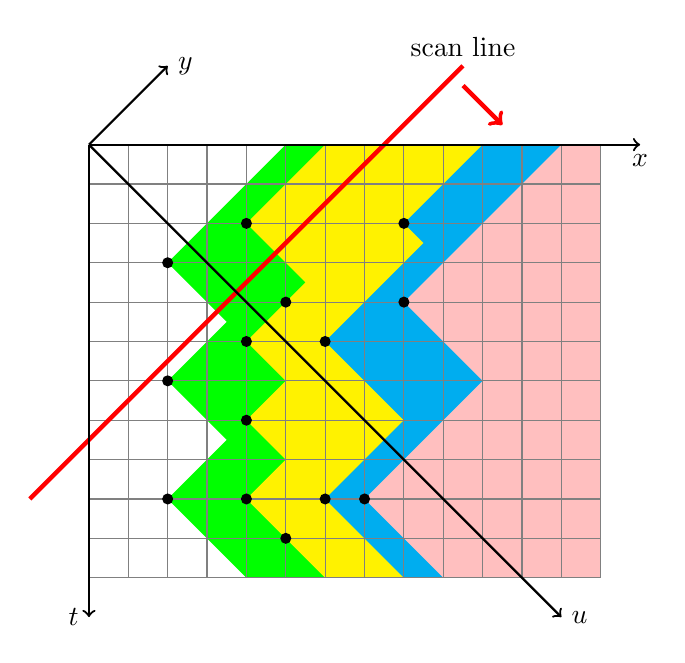
\begin{tikzpicture}

		\coordinate (corner1) at (6.5, 0  );
		\coordinate (corner2) at (6.5,-5.5);

		\coordinate (x11) at (1.0,-1.5);
		\coordinate (x12) at (1.0,-3.0);
		\coordinate (x13) at (1.0,-4.5);

		\coordinate (x21) at (2.0,-1.0);
		\coordinate (x22) at (2.0,-2.5);
		\coordinate (x23) at (2.0,-3.5);
		\coordinate (x24) at (2.0,-4.5);

		\coordinate (x31) at (2.5,-2.0);
		\coordinate (x32) at (2.5,-5.0);

		\coordinate (x41) at (3.0,-2.5);
		\coordinate (x42) at (3.0,-4.5);

		\coordinate (x51) at (3.5,-4.5);

		\coordinate (x61) at (4.0,-1.0);
		\coordinate (x62) at (4.0,-2.0);

		\fill [fill=green]
			(2.5,0.0)--(corner1)--(corner2)--(2.0,-5.5)--(x13)--+(0.75,0.75)--(x12)--+(0.75,0.75)--(x11);
		\fill [fill=yellow]
			(3.0,0.0)--(corner1)--(corner2)--(3.0,-5.5)--(x24)--+(0.5,0.5)--(x23)--+(0.5,0.5)--(x22)--+(0.75,0.75)--(x21);
		\fill [fill=cyan]
			(5.0,0.0)--(corner1)--(corner2)--(4.0,-5.5)--(x42)--+(1,1)--(x41)--+(1.25,1.25)--(x61);
		\fill [fill=pink]
			(6.0,0.0)--(corner1)--(corner2)--(4.5,-5.5)--(x51)--+(1.5,1.5)--(x62);

		\draw [help lines,thin,step=5mm] (0,-5.5) grid (6.5,0);

		\fill (x11) circle (2pt);
		\fill (x12) circle (2pt);
		\fill (x13) circle (2pt);

		\fill (x21) circle (2pt);
		\fill (x22) circle (2pt);
		\fill (x23) circle (2pt);
		\fill (x24) circle (2pt);

		\fill (x31) circle (2pt);
		\fill (x32) circle (2pt);

		\fill (x41) circle (2pt);
		\fill (x42) circle (2pt);

		\fill (x51) circle (2pt);

		\fill (x61) circle (2pt);
		\fill (x62) circle (2pt);

		\coordinate (scanlineend) at (4.75,1);
		\draw[ultra thick,red,->] (4.75,0.75)--+(0.5,-0.5);
		\node at (scanlineend) [above] {scan line};
		\draw[ultra thick,-,red] (scanlineend)--+(-5.5,-5.5);

		\draw[thick, ->] (0,0) -- (7, 0) node [below] {$x$};
		\draw[thick, ->] (0,0) -- (1, 1) node [right] {$y$};
		\draw[thick, ->] (0,0) -- (0,-6) node [left]  {$t$};
		\draw[thick, ->] (0,0) -- (6,-6) node [right] {$u$};
	\end{tikzpicture}

	\caption{$t$-$x$ 平面上に描いた巡査達の軌跡 \label{fig:uyspace}}
\end{figure}


初めに scanline 全体を色 $c_0$ で塗る.

scanline が点 $a_1$ に重なったとき,
scanline の $y > y_1$ の部分を色 $c_1$ で塗る.
次に scanline が $a_2$ に重なったとき,
$y_2$ が scanline の色 $c_0$ の範囲(境界は含まれる)にあれば
$y_2 \leq y \leq y_1$ と点 $a_2$ を色 $c_1$ で塗る.
$y_2$ が scanline の色 $c_1$ の範囲にあれば
$y \geq y_2$ と点 $a_2$ を色 $c_2$ で塗る.


このように,
scanline を動かしていって新たに重なる点 $a_i$ が scanline の
色 $c_k$ の部分にあれば,$y_i$ から色 $c_{k + 1}$ で塗られた部分まで
(無ければ $y = \infty$ まで)色 $c_{k + 1}$ で塗ることを繰り返していく.
このように点と重なるごとに更新されていく scanline の色で $t$-$x$ 平面を塗り分けていくことで
平面上のそれぞれの色 $c_i$ の領域が
$\dbigcup_{a \in B(X_i)} R(a) \setminus \dbigcup_{a \in B(X_{i + 1})} R(a)$
を表すことになり,
$\dbigcup_{a \in B(X_i)} L(a)$ の境界線上を各巡査が動けばよいことが分かる.

scanline の色として説明した部分は,
scanline の色に対応する区間を管理すればよく,
平衡二分木を用いて,各点と重なる毎に $O(\log N)$ で検索・追加をすれば,
合計 $O(N \log N)$ で平面の塗り分けが完了する.
ソートと合わせた全体の計算量は $O(N \log N)$ となる.
scanline は各点を通る時点で
各点を担当する巡査の番号と軌跡が決められるので,
随時必要な情報を出力していくことができる.
これにより必要な巡査の数を知ることができるのも明らかである.

\begin{coro}
	$G$ が Line,
	巡査が1人または複数で,
	最初の訪問時刻が指定されており,以降周期ちょうど毎の時刻に訪問しなければならないとき,
	$N := \dsum_{i = 1}^n \dfrac{lcm(q_1, \ldots, q_n)}{q_i}$
	% ( $lcm$ は最小公倍数)
	として $O(N \log N)$ で必要な巡査の数とその軌跡を計算できる.
\end{coro}

これは $lcm(q_1, \ldots, q_n)$ 時間周期で繰り返しとなるので明らかである.





\section{UStar}

Star では巡査1人で利得と{\timelimit}がすべて等しい場合を除き \decisionpp はNP困難であったが,
UStar の場合は{\timelimit}がすべて等しければ巡査が複数で \optpp でも多項式時間アルゴリズムが存在する.


\subsection{{\timelimit}がすべて等しい場合}

% \subsubsection{巡査が1人の場合}

% UStarでは{\timelimit}がすべて等しいときはすべての頂点の訪問のコストが等しいので,
% 利得の大きい順に選ぶことで最適解が得られる.
% 1つの頂点を訪問するのに $2d$ の時間がかかり,合計で $Q$ 以内でなければならないので,
% 選ぶ個数は $\lrfloor{\dfrac{Q}{2d}}$ 個となり,
% ヒープソートなどを用いれば $O\lr{n + \lrfloor{\dfrac{Q}{2d}} \log n}$ の時間で解くことができる.


% 利得がすべて等しいときは $q_i$ の大きいものから順に選べばよいことだけは言える.
% なぜならば,警備している点の集合 $V_s$ について,
% $x_i \in V_s$ と $x_j \in V \setminus V_s$ であって
% $q_i < q_j$ となる組が存在すれば,
% 辺の長さがすべて同じなので $x_i$ を訪問する時間で代わりに $x_j$ を訪問することができ,
% $q_i < q_j$ であるからそれ以外の時間は元の巡査の動きをそのまま用いることができるためである.
% こうして得られる警備する点の集合 $V_s \cup \set{ x_j} \setminus \set{ x_i }$ の利得は
% 元の利得以上となる.
% しかし,$q_i$ の大きいものからいくつ選べるかは自明ではなく,未解決.



% \subsubsection{巡査が複数の場合}
% % 

% Star の複数人の巡査による警邏はNP困難であったが,
% UStar の場合{\timelimit}がすべて等しいならば多項式時間アルゴリズムが存在する.

\begin{theo}
	\label{theo:3_UStar_multiple_Q_polytime}
	$G$ が UStar で{\timelimit}がすべて等しい場合,
	巡査が複数で \optpp でも
	多項式時間アルゴリズムが存在する.
\end{theo}

\begin{proof}[証明]
この場合,点の訪問のコストがすべて等しいことから,
利得の大きいものから選べばよいことは明らかであるが,
ちょうど $\lrfloor{\dfrac{mQ}{2d}}$ 点を警備する警邏を以下のように構成できる.

まず,利得の大きいものから $\lrfloor{\dfrac{mQ}{2d}} (=: l)$ 点を求め,
$v_1', v_2', \ldots, v_l'$ とする 
$(p_1' \geq p_2' \geq \cdots \geq p_l')$.

最初に巡査 $s_1$ が時刻 $t_0$ に原点を出発して
$v_1', v_2', \ldots, v_l'$ を順番に速さ$1$ で動きながら訪問していく.
巡査 $s_i$ は時刻 $t_0 + (i - 1)Q$ に原点を出発し,
$s_1$ より $(i - 1)Q$ だけ遅れて同じ動きをする.
各巡査が原点を出発して $v_1', \ldots, v_l'$ を訪問し
再び原点に戻るまでの時間は $2dl$ であり,
$2dl = 2d \lrfloor{\dfrac{mQ}{2d}} \leq mQ$ であるから,
時刻 $t_0 + (i - 1)Q$ に原点を出発した巡査 $s_i$ は
時刻 $t_0 + (i - 1)Q + mQ$ までには $v_l'$ まで訪問して原点に戻っており,
時刻 $t_0 + (i - 1)Q + mQ$ に原点を出発して再び同じ動きを繰り返すことができる.

このような動きを繰り返すことで,どの点 $v_i'$ についてもちょうど $Q$ おきに
巡査が訪問しているため,$v_1, \ldots, v_l'$ を警備できている.

一方,$m$ 人の巡査が警備できる点は高々 $\lrfloor{\dfrac{mQ}{2d}}$ 点であることが示せる.
任意の長さ $Q$ の時間 $[t_0, t_0 + Q]$ を切り取って考える.
警備している頂点集合を $V_S$ とすると,
$V_S$ のすべての頂点は少なくとも1回はこの時間に訪問されなければならない.
すると,各頂点 $v_i \in V_S$ に対して
$[t_0, t_0 + Q]$ のうち少なくとも $2d$ の時間は
$v_i$ に対応する辺 $e_i$ に巡査は存在しなければならない.
なぜならば,
(1) ある巡査が時間 $[t_0 + d, t_0 + Q - d]$ に $v_i$ を
1度以上訪問している場合,
少なくともその前後 $2d$ の時間はその巡査は辺 $e_i$ 上に存在しなければならず,
またこの時間は $[t_0, t_0 + Q]$ に含まれており,
(2) 時間 $[t_0 + d, t_0 + Q - d]$ に $v_i$ が1度も訪問されていない場合,
$[t_0, t_0 + d)$ か $(t_0 + Q - d, t_0 + Q]$ の少なくとも一方で訪問されるはずだが,
$[t_0, t_0 + d)$ に訪問されるならば $v_i$ にいた最後の時刻を $t_e$ として
$t_e + Q$ までにもう一度は訪問されるはずであり,
その時刻は $[t_0 + d, t_0 + Q - d]$ に含まれない場合を考えているので,
少なくとも $[t_0, t_e + d]$ と $[t_e + Q - d, t_0 + Q]$ の時間は
どれかの巡査が $e_i$ に存在しており,この時間は合わせて $2d$ となり,
いずれの場合も $2d$ の時間は $v_i$ の訪問のために使っている.
$(t_0 + Q - d, t_0 + Q]$ の場合も同様である.
% ことを以下のように示すことができる.
% 任意の点 $v_i \in V_S$ について,
% 時間 $[t_0, t_0 + Q]$ に少なくとも1回 $v_i$ はいずれかの巡査により訪問される.
% \begin{itemize}
% \item
% ある巡査が時間 $[t_0 + d, t_0 + Q - d]$ に $v_i$ を
% 1度でも訪問しているとき
% (いずれかの巡査が $v_i$ に存在する時刻が
% $[t_0 + d, t_0 + Q - d]$ の中にあるとき),
% 少なくともその前後 $2d$ の時間はその巡査は辺 $e_i$ 上に存在しなければならず,
% またこの時間は $[t_0, t_0 + Q]$ に含まれている.
% \item 
% $v_i$ が $[t_0 + d, t_0 + Q - d]$ に1度も訪問されないときは,
% $[t_0, t_0 + d)$ または $(t_0 + Q - d, t_0 + Q]$ に少なくとも1度訪問される.
% $[t_0, t_0 + d)$ に訪問される場合,点 $v_i$ に巡査が存在した
% 最後の時刻を $t_e \in [t_0, t_0 + d)$ とすると,
% $t_e + Q$ までに再び $v_i$ は訪問されるはずである.
% $[t_e, t_0 + Q - d]$ に再び訪問されることはない場合を考えているので,
% 再度訪問される時刻は $[t_0 + Q - d, t_e + Q]$ に含まれることになる.
% すると,巡査は $[t_0, t_e + d] \cup [t_e + Q - d, t_0 + Q]$ の間は
% 辺 $e_i$ に存在することになるので,
% $[t_0, t_0 + Q]$ の間に合計で少なくとも
% $(t_e + d - t_0) + (t_0 + Q - (t_e + Q - d)) = 2d$ の時間
% 巡査は辺 $e_i$ に存在することになる.
% $(t_0 + Q - d, t_0 + Q]$ の場合も対称なので同様に考えればよい.
% \end{itemize}
% 以上により示された.
すると,$m$ 人の巡査で $V_S$ の点を訪問するとき
巡査が使える時間は合計 $mQ$ であるので,
$2d \cdot |V_S| \leq mQ$ である必要があり,
これにより $|V_S| \leq \lrfloor{\dfrac{mQ}{2d}}$ が言える.

以上から $\lrfloor{\dfrac{mQ}{2d}}$ 点の警邏が最適解であることが分かり,
ヒープソートなどを用いれば
$O\lr{n + \lrfloor{\dfrac{mQ}{2d}} \log n}$ の時間で解くことができる.
これで定理\ref{theo:3_UStar_multiple_Q_polytime}が示された.
\end{proof}





\subsection{{\timelimit}が一般の場合}

UStar で{\timelimit}がすべて等しい場合には多項式時間アルゴリズムが示せたが,
{\timelimit}が一般の場合は計算量を決定できなかった.%未解決である.
% 巡査が1人で利得がすべて等しいときは $q_i$ の大きいものから順に選べばよいことだけは言えるが,
% それでも $q_i$ が大きいものからいくつの頂点が警邏できるかは自明でなく,未解決である.
そこで,ここでも
Line のときのように,
最初の訪問時刻からその{\period}ごとの時刻は必ず訪問しなければならないという問題をここでも考えてみる.


\subsubsection{最初の訪問時刻指定,周期ちょうど毎に訪問}

% {\timelimit}の代わりに{\period}と最初の訪問時刻 $r_i$ が与えられたときに,
% 最初の訪問時刻からその{\period}ごとの時刻は必ず訪問しなければならないという制約の問題の場合,
% \decisionpp は巡査が1人ならば多項式時間アルゴリズムが存在する.


\begin{theo}
	\label{theo:4_UStar_single_exact_starttime}
	$G$ が UStar で巡査が1人,
	最初の訪問時刻と{\period}が与えられたときに,
	最初の訪問時刻からその{\period}ごとの時刻は必ず訪問しなければならないという制約の場合,
	{\period}は異なっていても
	\decisionpp には多項式時間アルゴリズムが存在する.
\end{theo}

\begin{proof}[証明]
	各頂点 $v_i$ を訪問しなければならない時刻は $q_i k + r_i \; (k \in \Z)$ として与えられる.
	全 $n$ 点に対するこれらの和集合を
	$T := \dbigcup_{i = 1}^n \setmid{q_i k + r_i }{ k \in \Z }$ 
	とおくと,
	\decisionpp が Yes である(=全点を警備できる)ことと,
	連続した訪問しなければならない時刻の差が移動時間 $2d$ 以上であること,すなわち
	$T$ に含まれるどの2つの整数も差が $2d$ 以上であることが同値であることが分かる.
	これは
	% $gcd(\wc,\wc)$ を最大公約数として,
	任意の2点 $v_i, v_j \in V$ と
	任意の整数 $k,l$ に対して $\abs{ (q_i k + r_i ) - (q_j l + r_j) } \geq 2d$
	となり,これは
	任意の整数 $n$ に対して $\abs{ (r_i - r_j) + gcd(q_i, q_j) n } \geq 2d$
	と同値であり,
	左辺の最小値を考えると
	$\abs{ r_i - r_j }$ を $gcd(q_i, q_j)$ で割った余り $a$ と
	$gcd(q_i, q_j) - a$ のうち小さい方が $2d$ 以上かをチェックすればよい.
	この計算は定数時間であり
	${}_n C_2$ 通りこれを試せばよいので全体で多項式時間となる.
\end{proof}

\decisionpp で巡査を複数とすると,$T$ に差が $2d$ 未満の整数が含まれていても
複数の巡査によりそれぞれ訪問できる場合が生じる.
$m$ 人の巡査がいるので,任意の $t \in T$ に対し $[t, t + 2d)$ の時間に
含まれる $T$ の時刻が $m$ 個以下であれば全点を訪問でき,
$m + 1$ 以上となる $t$ が存在すれば $m$ 人の巡査により訪問できない点が1つ以上生じる.
これは $T$ に含まれる整数の分布の情報を知る必要があるが,
効率的なアルゴリズムは見つけられなかった.



\decisionpp では巡査が1人ならば多項式時間アルゴリズムが存在したが,
一方 \optpp は巡査が1人でも(複数人でも)NP困難となる.

\begin{theo}
	\label{theo:5_UStar_exact_starttime_NPhard}
	$G$ が UStar で,
	最初の訪問時刻と{\period}が与えられたときに,
	最初の訪問時刻からその{\period}ごとの時刻は必ず訪問しなければならないという制約の場合,
	巡査が1人で利得がすべて等しい場合でも,
	\optpp はNP困難である.
\end{theo}


\begin{proof}[証明]
	最大独立点集合問題からの帰着による.

	最大独立点集合問題は,
	無向グラフ $G' = (V', E')$ と自然数 $M$ が与えられたときに
	独立点集合でサイズが最大のものを求める問題でNP完全であることが知られている.
	この問題において,2点間に辺の存在する $v_i, v_j \in V'$ を両方選ぶことはできないということを,
	\optpp において2点のどちらか一方しか警備できないという状況を作ることで表現する.

	まず簡単のため $d = 1/2$ とする.
	これにより巡査がちょうど速さ $1$ で動くとすると各頂点の訪問にかかる時間は $1$ となり,
	UStar なのですべての整数の時刻にどれか1点を訪問できる.
	その上で,周期 $q_i$, 最初の訪問時刻 $r_i$ は整数,$p_i = 1$ とする.
	\optpp の UStar の点集合 $V$ は $V'$ のサイズと同じとし,以降同じ添え字で対応させる.
	点 $v_i \in V$ を警備するために訪問しなければならない時刻の列は
	$q_i k + r_i \; (k \in \N)$ で表される.
	すると,$v_i$ と $v_j$ の両方を警備できる必要十分条件は
	$q_i k + r_i = q_j l + r_j$ , 移項すると
	$r_i - r_j = q_j l - q_i k$ 
	となる自然数 $k, l$ が存在しないこととなるが,
	これは $r_i - r_j = gcd(q_i,q_j) n$ となる整数 $n$ が存在しないことと同値である.
	% 実際,
	% $r_i - r_j = q_j l - q_i k$ となる自然数 $k,l$ が存在するとき,
	% $gcd(a,b)$ を $a$ と $b$ の最大公約数として,
	% $n = \dfrac{q_j}{gcd(q_i,q_j)} l - \dfrac{q_i}{gcd(q_i,q_j)} k$ とすれば
	% $r_i - r_j = gcd(q_i,q_j) n$ であり,
	% 逆に $r_i - r_j = gcd(q_i,q_j) n$ となる整数 $n$ が存在するとき,
	% $gcd(q_i,q_j) = q_i l' + q_j k'$ を満たす整数の組 $l'$, $k'$ が存在することは
	% ユークリッド互除法より言えるので,$l = nl'$, $k = -nk'$ とすると
	% $r_i - r_j = q_j l - q_i k$ となる.
	% まとめると,
	よって,
	$v_i$ と $v_j$ の両方を警備できる必要十分条件は
	$r_i \not\equiv r_j \mod gcd(q_i, q_j)$
	となる.

	ここで,${}_n C_2$ 個の相異なる素数 $p_{ij} (1\leq i < j \leq n)$ を用意し,
	各頂点の周期を
	$q_i = p_{1i} p_{2i} \cdots p_{(i - 1)i} p_{i(i + 1)} \cdots p_{i,n}$
	とすると,$gcd(q_i,q_j) = p_{ij}$ ($i < j$ のとき)となり,
	先ほどの条件は
	$r_i \not\equiv r_j \mod p_{ij}$
	となる.

	$G'$ において
	$(v_i', v_j') \in E'$     ならば $r_i \equiv r_j \equiv 0 \mod p_{ij}$,
	$(v_i', v_j') \not\in E'$ ならば $r_i \equiv 0, r_j \equiv 1 \mod p_{ij}$
	と定めると,
	各 $r_k$ に対して相異なる $n - 1$ 個の素数で割ったときの余りが与えられるので,
	中国剰余定理からそのような $r_k$ がその $n - 1$ 個の素数の積 $q_k$ を法として一意に存在することが言え,
	これにより,$(v_i', v_j') \in E'$ ならば $r_i \equiv r_j \mod p_{ij}$
	$(v_i', v_j') \not\in E'$ ならば $r_i \not\equiv r_j \mod p_{ij}$
	を満たすように各 $r_k$ を定めることができる

	最後に,${}_n C_2$ 個の相異なる素数を用意する計算量も確かめる必要がある.
	$k$ 番目に小さい素数を $P_k$ と書くと,$k \geq 6$ のときは
	$P_k < k( \ln k + \ln\ln k )$ であることが知られているため~\cite{dusart1999k},
	$k( \ln k + \ln\ln k )$ までの自然数を順に素数かどうか判定していくことで
	$k$ 個以上の素数を得ることができる.
	ある数が素数であるかどうかを判定する多項式時間アルゴリズムは存在するので~\cite{agrawal2004primes},
	${}_n C_2$ 個の素数の列挙は $n$ の多項式時間でできる.

	以上の手順で $q_k$ と $r_k$ を設定することにより,
	$G'$ においてサイズ最大の独立点集合を求める問題を,
	巡査1人, $G$ が UStar,
	最初の訪問時刻が指定され周期ちょうど毎に訪問しなければならない制約での \optpp に帰着できた.
	以上より定理\ref{theo:5_UStar_exact_starttime_NPhard}は示された.
\end{proof}



\subsubsection{周期ちょうど毎に訪問}
今,最初の訪問時刻と周期が指定された場合を考えたが,
周期のみが指定されている場合は \decisionpp でもNP困難となる.

\begin{theo}
	\label{theo:6_UStar_exact_NPhard}
	$G$ が UStar で,
	{\period}のみ与えられたときに,
	最初の訪問時刻からその{\period}ごとの時刻は必ず訪問しなければならないという制約の場合,
	% 周期ちょうど毎の時刻に訪問しなければならないとき,
	巡査が1人で \decisionpp でもNP困難である.
\end{theo}

\begin{proof}[証明]
	Disjoint Residue Class Problem からの帰着による.

	ある整数のペアの集合 $\set{ (m_1, r_1), \ldots, (m_n, r_n) }$ が
	Disjoint Residue Class であるとは,
	任意の整数 $x$ に対して $x \equiv r_i \mod m_i$ となるような $i$ が
	高々1つ存在することと定義する.
	Disjoint Residue Class Problem とは
	整数の組 $(m_1, \ldots, m_n)$ が与えられたときに,
	$\set{ (m_1, r_1), \ldots, (m_n, r_n) }$ が
	Disjoint Residue Class となるような組 $(r_1, \ldots, r_n)$ が
	存在するかを判定する問題であり,
	これはNP困難であることが示されている~\cite{kawamura2015simple}.

	Disjoint Residue Class Problem は,巡査1人, $G$ が UStar, $p_i = 1$ で
	{\period}ごとの時刻は必ず訪問しなければならないという制約での \decisionpp に多項式時間帰着できる.
	Disjoint Residue Class Problem の入力が $(m_1, \ldots, m_n)$ のとき,
	UStar で $V = \set{ v_1, \ldots, v_n }$, $q_i = m_i$, $d = 1/2$ とする.
	$d = 1/2$ より整数の時刻にいずれかの点を訪問できるようにする.
	各頂点 $v_i$ の最初の訪問時刻を $r_i$ とすると,
	この点を警備するために訪問しなければならない時刻の列は
	$q_i k + r_i (k \in \N)$ で与えられるが,
	全点を警備するためには任意の2点 $v_i, v_j \in V$ , 任意の整数 $k,l$ について
	$q_i k + r_i \neq q_j l + r_j$
	である必要がある.
	Disjoint Residue Class Problem の解 $(r_1, \ldots, r_n)$ が存在するならば,
	これにより任意の時刻 $t \in \Z$ に対して $t \equiv r_i \mod q_i$, 
	すなわち $t = r_i + q_i k$ となる $k \in \Z$ が存在するような $i$ は高々1つであり,
	任意の $k,l \in \Z$ に対して $q_i k + r_i \neq q_j l + r_j$ が成り立つので,
	巡査は全点を警備できる.
	よって,Disjoint Residue Class Problem が Yes ならばこの \decisionpp も Yes となる.

	逆に,\decisionpp の解が存在するとき,
	全点を警備できるのでその警邏において各頂点 $v_i$ を最初に訪問する時刻を $r_i$ とすると,
	任意の $v_i,v_j \in V$, $k,l \in \Z$ に対し
	\begin{equation}
		\label{eq:patroll_disjoint}
		q_i k + r_i \neq q_j l + r_j
	\end{equation}
	が成り立つ.すると,任意の時刻 $t \in \Z$ に対して
	$t \equiv r_i \mod q_i$ となるような $i$ が2つ存在するとすると,
	それを $i$, $j$ として
	$t \equiv r_i \mod q_i$, $t \equiv r_j \mod q_j$
	すなわち,ある整数 $k,l$ が存在して
	$t = q_i k + r_i$, $t = q_j l + r_j$
	となり,この $k,l$ によって
	$q_i k + r_i = q_j l + r_j$ となり,式\ref{eq:patroll_disjoint} に矛盾する.
	よって,任意の整数 $t$ に対して $t \equiv r_i \mod q_i$ を満たす
	$i$ は高々1つであるような $r_i$ が与えられたので,
	\decisionpp が Yes ならば Disjoint Residue Class Problem も Yes となる.

	以上より定理\ref{theo:6_UStar_exact_NPhard}は示された.
\end{proof}


